%%%%%%%%%%%%%%%%%%%%%%%%%%%%%%%%%%%%%%%%%%%%%%%%%%%%%%%%%%%%%%%%%%%%%%%%%%
\chapter{Nástroj pro optimalizaci velikosti bajtkódu}\label{Jbyco}

% TODO 
% * zmínit, že záleží na pořadí, a že každá optimalizace produkuje další možnosti k optimalizaci, mebo taky ne

V~této kapitole popisuji návrh a implementaci nástroje \texttt{jbyco} nebo-li Java Bytecode Optimizer určeného k~optimalizaci velikosti \texttt{class} souborů. Nástroj implementuje optimalizační metody, které jsem navrhla v~předchozí kapitole. Efektivita těchto metod je na základě výstupů programu vyhodnocena v~kapitole \ref{Jbyco:Results}.

\section{Požadavky na program}\label{Jbyco:Requirements}

Cílem programu je implementovat navržené optimalizační metody a na testovacím vzorku \texttt{class} souborů demonstrovat jejich efektivitu. %Jedním z~požadavků je proto i návrh vhodného programového rozhraní, který umožní snadno implementovat nové optimalizační metody. 
Vstupem programu může být \texttt{class} soubor, \texttt{jar} soubor nebo adresář. Výstupem pak bude optimalizovaný \texttt{class soubor}, nebo kopie souborů s~optimalizovanými \texttt{class} soubory. Každý \texttt{class} soubor se bude zpracovávat nezávisle na dalších souborech a informacích. Dále je potřeba umožnit vypisovat informace o~provedených optimalizacích.

\section{Návrh programu}\label{Jbyco:Design}

Kapitola \ref{Optimization:Methods} je ve velké míře věnovaná optimalizačním metodám založeným na náhradě sekvencí instrukcí. Rozhodla jsem se proto na tyto metody zaměřit i při implementaci. Metody lze rozdělit na tzv. peephole optimalizace a optimalizace toku programu. Peephole optimalizacím se dále věnuji v~kapitole \ref{Jbyco:Design:Peephole}, zatímco optimalizacím toku programu v~kapitole \ref{Jbyco:Design:Flow}. 

K~implementaci jsem se rozhodla použít knihovnu ASM. Avšak s~ohledem na to, jakým způsobem je v~knihovně bajtkód reprezentován, je výhodné hned na počátku optimalizací odstranit informativní atributy. Tyto atributy by jinak byly součástí seznamů instrukcí, což by zkomplikovalo vykovávání dalších optimalizací. 

Dále jsem se rozhodla ve zjednodušené formě aplikovat realokaci lokálních proměnných. Toto zjednodušení spočívá v~přečíslení indexů lokálních proměnných tak, aby byly proměnné očíslovány v~pořadí prvního užití v~instrukcích. Tímto přeskupením může vzniknout kompaktnější pole lokálních proměnných. Takový nástroj navíc poskytuje přímo knihovna ASM. Nad celkovým pořadím žádaných optimalizací se zamýšlím v~kapitole \ref{Jbyco:Design:Ordering}.

\subsection{Peephole optimalizace}\label{Jbyco:Design:Peephole}

Většina navržených optimalizačních metod v~kapitole \ref{Optimization:Methods} je založených na nalezení vzorové sekvence instrukcí a náhradě této sekvence za optimalizované řešení. Tento způsob optimalizace se dle McKeemana \cite{McKeeman:Peephole} nazývá peephole optimalizace a je specifický tím, že se vždy zkoumá jen malý úsek kódu. Nezbytnou součástí návrhu programu \texttt{jbyco} je tedy i návrh rozhraní pro peephole optimalizace. Konkrétně je třeba navrhnout, jakým způsobem budou definovány vzorové sekvence, jak budou vzorové sekvence rozpoznávány v~kódu určeném k~optimalizaci a jak bude probíhat samotná úprava kódu.

Způsobů implementace peephole optimalizace je mnoho \cite{Chakraborty:Peephole}. Jako přímé řešení se nabízí převádět vstupní bajtkód na řetězcovou reprezentaci. Vzorové sekvence by pak byly popsány regulárními výrazy a problematika nalezení a úpravy bajtkódu by se zjednodušila na prosté hledání a nahrazování regulárních výrazů v~řetězci. Na závěr by bylo nutné řetězcovou reprezentaci opět převést na sekvenci instrukcí. Výhodou tohoto přístupu je snadné ladění, neboť řetězcová reprezentace kódu je snadno čitelná.

Efektivnější variantou by mohlo být hledání regulárními výrazy přímo nad instrukcemi bajtkódu. Regulární výrazy pro popis vzorových sekvencí by bylo možné předzpracovat a vygenerovat konečný stavový automat, který bude tyto výrazy rozpoznávat. Nalezené sekvence instrukcí pak mohou být nahrazeny za optimální. Pokud bude automat generován v~době překladu, pak by takové řešení mělo být velice rychlé. Vyžaduje však implementovat nástroje pro lexikální a syntaktickou analýzu regulárních výrazů, nástroje pro převod regulárních výrazů na konečný automat a nástroje pro minimalizaci konečného automatu. Pokud se však sleví z~požadavků na sílu jazyka pro popis vzorových sekvencí, lze tuto variantu zjednodušit.

Většinu vzorových sekvencí v~navržených optimalizačních metodách tvoří posloupnost instrukcí konstantní délky. Vzorové instrukce jsou specifikovány svými operačními kódy a omezeními kladenými na jejich parametry. Jako možné řešení se proto nabízí definovat vzorové sekvence pomocí posloupností operačních kódů a teprve při nalezení odpovídající sekvence kontrolovat další omezení. Pokud jsou všechna omezení splněna, může být sekvence optimalizována. Ve své implementaci jsem zvolila tuto variantu. 

Každá peephole optimalizace je tedy definována posloupností symbolů, které reprezentují množiny operačních kódů, a akcí, které provádí dodatečné kontroly a optimalizaci. Jedním z~výstupů akce je informace o~tom, zda se optimalizace provedla či neprovedla.
Rozpoznávání posloupností symbolů lze realizovat jednoduchým konečným automatem, jehož stavy jsou indexy do posloupnosti symbolů. Počátečním stavem je nula a koncovým stavem je délka posloupnosti. Pokud operační kód instrukce na vstupu patří do množiny reprezentované symbolem na indexu určeném aktuálním stavem, automat provede přechod na následující index. Pokud automat přejde do koncového stavu, provede se pro nalezenou sekvenci instrukcí odpovídající akce.

\subsection{Optimalizace toku programu}\label{Jbyco:Design:Flow}

Některé z~navržených metod pro optimalizaci podmíněných a nepodmíněných skoků nelze implementovat pomocí peephole optimalizací, neboť vyžadují dodatečné informace o~návěštích a adresách instrukcí. Některé z~těchto optimalizací navíc mohou tyto informace zneplatnit, a proto je třeba je při každé možné změně aktualizovat. 
Adresy instrukcí stačí určit za použití heuristiky, kdy se adresy počítají pomocí největších možných velikostí instrukcí. Získané adresy tak popisují nejhorší možný případ.

\subsection{Pořadí optimalizačních metod} \label{Jbyco:Design:Ordering}

U~některých optimalizačních metod může záležet na pořadí, v~jakém se aplikují. Například metodu pro substituci číselných konstant má smysl uskutečnit až jako poslední krok optimalizace, neboť jiné metody by mohly tuto substituci zvrátit. Na druhou stranu metoda pro odstranění zbytečných atributů může usnadnit další manipulaci s~kódem a je proto vhodné ji aplikovat při načtení vstupního bajtkódu. 

U~optimalizací sekvencí instrukcí může docházet k~tomu, že některé optimalizace budou vytvářet příležitosti pro další optimalizace. Vzhledem k~uspořádání zásobníkového kódu pak může být výhodnější aplikovat metody pro sekvence instrukcí na kód v~opačném směru, tedy od poslední instrukce k~první. Nejprve se tak zkoumají operace a jejich parametry, předtím než se začnou zkoumat další vztahy mezi instrukcemi. Tento způsob práce s~bajtkódem lze podpořit expanzí duplikací. Pokud je možné instrukci pro duplikaci aplikovat na úrovni instrukcí kódu, může tato aplikace vytvořit nové příležitosti pro optimalizace.

Na pořadí metod má vliv i způsob, jakým budou optimalizační metody implementované. Knihovna ASM umožňuje kombinovat dva přístupy pro práci z~bajtkódem. Aby se zabránilo opakovanému generování stromové reprezentace, je vhodné optimalizaci rozdělit na tři fáze. V~první fázi je vstupní pole bajtů převedeno na stromovou reprezentaci. Během tohoto převodu lze pomocí zřetězení návštěvníků již aplikovat některé optimalizace. Ve druhé fázi se optimalizuje stromová reprezentace. A~ve třetí fázi je stromová reprezentace skrze zřetězené návštěvníky opět převedena na pole bajtů. V~tomto okamžiku lze rozhodnout, zda optimalizace měly na vstupní kód nějaký efekt. Pokud došlo k~redukci velikosti bajtkódu, lze všechny fáze zopakovat. Pokud k~redukci nedošlo, proces optimalizace se ukončí. Validitu výsledného bajtkódu lze na závěr ověřit nástrojem z~knihovny ASM.
Konečný návrh na pořadí optimalizačních metod je následující:

\begin{enumerate}
\setlength{\itemsep}{0pt}
\setlength{\parskip}{0pt}
%\item Čtení pole bajtů.
\item Odstranění zbytečných atributů.
\item Expanze duplikací.
%\item Vytvoření stromové reprezentace. 
\item Zjednodušení kódu.
%\item Procházení stromové reprezentace.
\item Redukce duplikací.
\item Realokace lokálních proměnných.
\item Substituce číselných konstant.
%\item Vytvoření pole bajtů.
\end{enumerate}


\section{Popis implementace}

Program jsem implementovala v~jazyce Java 8 za použití knihovny ASM 5.0\footnote{\texttt{http://asm.ow2.org/}} a tříd, které vznikly v~rámci implementace nástroje \texttt{jbyca}. Překlad a instalaci zajišťuje knihovna Gradle 2.7\footnote{\texttt{http://gradle.org/}}. Program nepodporuje vytváření \texttt{jar} souborů z optimalizovaných souborů a kopírování souborů, které nejsou typu \texttt{class}, do výstupní struktury.

V~balíčku \texttt{jbyco.optimization} je umístěná třída \texttt{Application} s~hlavní metodou \texttt{main}. Tato metoda zpracuje parametry a vstupní soubor předá iterátoru \texttt{BytecodeFilesIterator} z~balíčku \texttt{jbyco.io}. Pro každý nalezený \texttt{class} soubor se zavolá metoda \texttt{optimizeClassFile} třídy \texttt{Optimizer}. Ve třídě \texttt{Optimizer} jsou implementované všechny fáze optimalizace batjkódu. Ke sběru informací o~provedených optimalizacích slouží třída \texttt{Statistics}. Třídy implementující optimalizační metody pro expanzi kódu jsou umístěné v~podbalíčku \texttt{expansion}, třídy pro zjednodušení kódu jsou v~podbalíčku \texttt{simplification} a třídy pro redukci kódu jsou obsažené v~podbalíčku \texttt{reduction}. Různé obecné nástroje a třídy jsou umístěné v~podbalíčku \texttt{common}. 

\subsubsection{Reprezentace vzorových sekvencí a akcí}

Balíček \texttt{jbyco.optimization.peephole} obsahuje třídy pro implementaci a aplikaci peephole optimalizací. Rozhraní \texttt{Symbol} pro symboly reprezentuje množinu operačních kódů. Má jedinou metodu \texttt{match} s~parametrem \texttt{AbstractInsnNode} z~knihovny ASM, která vrací \texttt{true}, pokud operační kód dané instrukce patří do množiny reprezentované symbolem, jinak \texttt{false}. Toto rozhraní je implementováno výčtem \texttt{Symbols}, kde každý operační kód je reprezentován jedním symbolem a další symboly reprezentují skupiny operačních kódů se stejnými vlastnostmi. Vzorovou sekvenci lze definovat pomocí anotace \texttt{Pattern}, která obsahuje pole symbolů typu \texttt{Symbol}. Akce je reprezentovaná třídou implementující funkční rozhraní \texttt{PeepholeAction} a anotovanou anotací \texttt{Pattern}. Každá akce definuje metodu \texttt{replace} s~paramery: seznam instrukcí typu \texttt{InsnList} z~knihovny ASM a pole instrukcí typu \texttt{AbstractInsnNode}. Seznam instrukcí je aktuální reprezentací těla zpracovávané metody. Pole instrukcí pak obsahuje instrukce ze seznamu instrukcí a tvoří nalezenou sekvenci instrukcí. Pomocí prvků tohoto pole lze snadno provádět dodatečné kontroly a modifikovat seznam instrukcí. Návratová hodnota je typu \texttt{boolean} a značí, zda došlo k~modifikaci seznamu instrukcí. Třída \texttt{InsnUtils} z~balíčku \texttt{jbyco.optimization.common} slouží akcím jako knihovna užitečných funkcí.

\subsubsection{Hledání vzorových sekvencí a aplikace akcí}

Třída \texttt{PeepholeRunner} z~balíčku \texttt{jbyco.optimization.peephole} zapouzdřuje hledání vzorů a spouštění odpovídajících akcí. Její metoda \texttt{loadActions} načte akce a vzory a vytvoří pro ně konečné automaty reprezentované instancemi třídy \texttt{StateMachine}. Třída \texttt{StateMachine} obsahuje metody pro testování, zda lze přečíst vstupní instrukci, pro čtení vstupní instrukce, pro určení, zda je automat v~konečném stavu, a pro vykonání příslušné akce. 

Metoda \texttt{findAndReplace} třídy \texttt{PeepholeRunner} slouží k~hledání vzorů a spouštění akcí. Dokud v~daném seznamu instrukcí dochází ke změnám, tak se v~něm opakovaně vyhledává. Pro aktuální instrukci se nejprve ověří, zda nemůže být přečtena některým z~načtených konečných automatů. Pokud ano, je vytvořena kopie tohoto automatu a vložena do fronty běžících automatů. Tato fronta je následně dále zpracovávána. Pokud automat z~fronty běžících automatů přečte aktuální instrukci, pak ve frontě zůstává, a pokud ji nepřečte, je z~fronty odebrán. Přejde-li automat do koncového stavu, spustí se akce, a modifikuje-li akce seznam instrukcí, fronta běžících automatů se vyprázdní a vyhledávání vzorů se restartuje.

\subsubsection{Aplikace optimalizací programového toku}

Třídy pro implementaci a aplikaci optimalizací programového toku jsou umístěné v~balíčku \texttt{jbyco.optimization.jump}. Obdobně jako u~peephole optimalizací jsou optimalizační akce definované pomocí funkčních rozhraní \texttt{LabelAction}, \texttt{FrameAction}, \texttt{TableSwitchAction} a \texttt{LookupSwitchAction}. Tyto akce lze načíst a aplikovat pomocí tříd \texttt{LabelTransformer}, \texttt{FrameTransformer}, \texttt{TableSwitchTransformer} a \texttt{LookupSwitchTransformer} rozšiřujících abstraktní třídu \texttt{MethodTransformer} z balíčku \texttt{jbyco.optimization.common}.
Bajtkód je optimalizován pomocí zřetězení těchto tříd a třídy \texttt{JumpTransformer}. Tato třída rozšiřuje abstraktní třídu \texttt{ClassTransformer} z balíčku \texttt{jbyco.optimization.common}.
Data nezbytná pro provádění optimalizací se sbírají ve třídě \texttt{JumpCollector}. Informace o~návěštích se uchovávají v~instancích třídy \texttt{LabelNodeInfo} a informace o~rámcích zásobníkových map ve \texttt{FrameNodeInfo}.

\section{Překlad a spuštění}

Nástroj je implementován v~programovacích jazyce Java 8. K~překladu a spuštění proto vyžaduje instalaci Java JDK 8 a Java JRE 8. Zdrojové soubory nástroje \texttt{jbyco} jsou součástí projektu \texttt{optimization}. Projekt lze přeložit a nainstalovat pomocí skriptu \texttt{gradlew} nástroje Gradle stejným způsobem, jako bylo popsáno v~kapitole \ref{Jbyca:Run}. Nástroj lze spustit příkazem \texttt{./jbyco}. Nápovědu vypíše volba \texttt{---help}.

% nástroj pro porovnání dvou souborů

\section{Zhodnocení výstupů programu}\label{Jbyco:Results}

Pomocí programu \texttt{jbyco} jsem optimalizovala vzorek dat, který jsem analyzovala v~kapitole \ref{Optimization:Analysis}. Jak je ukázáno v~tabulce \ref{tab:methods}, nejčastěji se prováděly optimalizační metody založené na náhradě sekvencí instrukcí pro práci se zásobníkem. Naopak nejméně se využívaly metody pro zjednodušování algebraických výrazů. V~tabulce chybí optimalizační metody, které se prováděly vždy a jejich aplikaci tedy nelze nijak kvantifikovat.

\begin{figure}
\begin{center}
  \begin{tabular}{r l} \hline
  \textbf{Počet náhrad} & \textbf{Optimalizační metoda} \\\hline

352 972	&	Optimalizace práce se zásobníkem	\\
167 242	&	Optimalizace podmíněných a nepodmíněných skoků	\\
123 173	&	Expanze duplikace	\\
34 934	&	Redukce duplikace	\\
32 528	&	Optimalizace konverze hodnot	\\
32 357	&	Optimalizace konkatenace řetězců	\\
2 788	&	Optimalizace práce s~objekty	\\
1 881	&	Zjednodušení algebraických výrazů	\\\hline

  \end{tabular}
\end{center}
\caption{Četnosti optimalizačních metod.}
\label{tab:methods}
\end{figure}

Vliv optimalizačních metod na celkovou velikost \texttt{class} souborů znázorňuje tabulka \ref{tab:sizes}. Je patrné, že nejefektivnější metodou bylo odstranění zbytečných atributů. Aplikace této metody přinesla úsporu 22,487\%. Z~metod pro optimalizaci instrukcí byla nejefektivnější optimalizace skoků s~1,741\%. Zajímavé je, že navzdory předpokladům má expanze duplikací negativní vliv na výslednou velikost. Při aplikaci optimalizací bez expanzí byla výsledná velikost souborů menší než při aplikaci optimalizací s~expanzí. Na základě tohoto zjištění tedy lze fázi expanze z~optimalizačního procesu odstranit.

\begin{figure}
\begin{center}
  \begin{tabular}{l r r} \hline

\textbf{Optimalizační metoda}	&	\textbf{Úspora v~B}	&	\textbf{Úspora v~\%}	\\\hline
Realokace lokálních proměnných					&	22 963	&			0,013	\\
Substituce číselných konstant					&	141 781	&			0,075	\\
Nahrazení sekvencí instrukcí					&	395 646	&			0,208	\\
Optimalizace skoků					&	3 313 415	&			1,741	\\
Odstranění zbytečných atributů			&	42 815 740			&	22,487			\\
Všechny optimalizace			&	46 886 770			&	24,626			\\
Všechny optimalizace bez expanze duplikací			&	46 888 858			&	24,627			\\\hline

  \end{tabular}
\end{center}
\caption{Vliv optimalizačních metod na celkovou velikost \texttt{class} souborů.}
\label{tab:sizes}
\end{figure}
          
Optimalizované \texttt{class} soubory jsem znovu analyzovala nástrojem \texttt{jbyca}. Optimalizace nijak výrazně neovlivnila maximální hloubky zásobníků operandů ani maximální počty lokálních proměnných. Na využití parametrů metody se optimalizace též nijak zásadně neprojevila. Zaznamenatelná změna však nastala u využití lokálních proměnných. Graf \ref{fig:cmp_locals} zobrazuje, kolik operací se v metodách průměrně provedlo s lokální proměnnou na daném indexu před a po optimalizaci. Obecně lze říci, že počet operací s proměnnými klesl, neboť proměnné na indexech větších než 80 využívá méně než 10 metod. Zvýšení počtu operací u některých proměnných s indexy v rozsahu 80 až 120 lze vysvětlit nahrazením instrukce \texttt{tableswitch} nebo \texttt{lookupswitch} za sekvenci podmíněných skoků, kde se porovnávaná hodnota opakovaně načítá z lokální proměnné. 

\begin{figure}[h!]
\centering
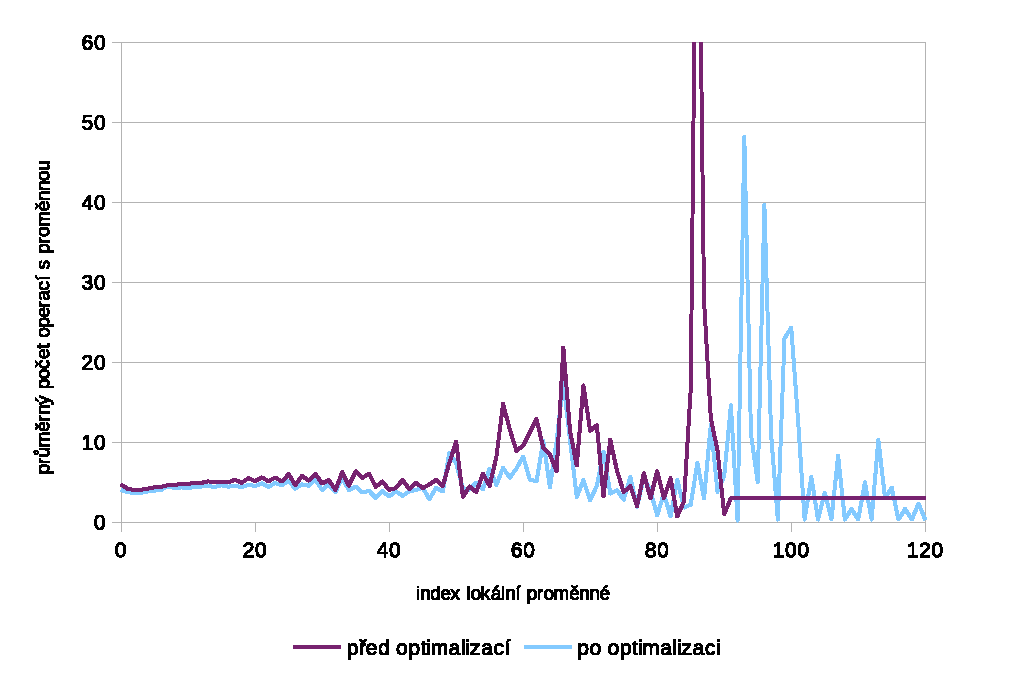
\includegraphics[scale=0.9]{fig/locals_comparison}
\caption{Využití lokálních proměnných před a po optimalizaci.}\label{fig:cmp_locals}
\end{figure}

Na grafu \ref{fig:cmp_size} je znázorněna změna celkových velikostí položek ve zpracovaných \texttt{class} souborech. Graf potvrzuje, že optimalizace měla největší vliv na velikost atributů. Celkem se ušetřilo 44,7 MiB ze 181,6 MiB.

Dosažené výsledky nejsou zanedbatelné, ale rozšířením optimalizačních metod by se mohlo dosáhnout ještě větší úspory paměti. Výhodou nástroje \texttt{jbyco} je však zachování původních struktur programů a snadná optimalizace souborů bez složité konfigurace. Jiné nástroje pro optimalizaci velikosti \cite{ProGuard} navíc ke své činnosti vyžadují vyřešené všechny závislosti mezi soubory, což nástroj \texttt{jbyco} nevyžaduje.


\begin{figure}[h!]
\centering
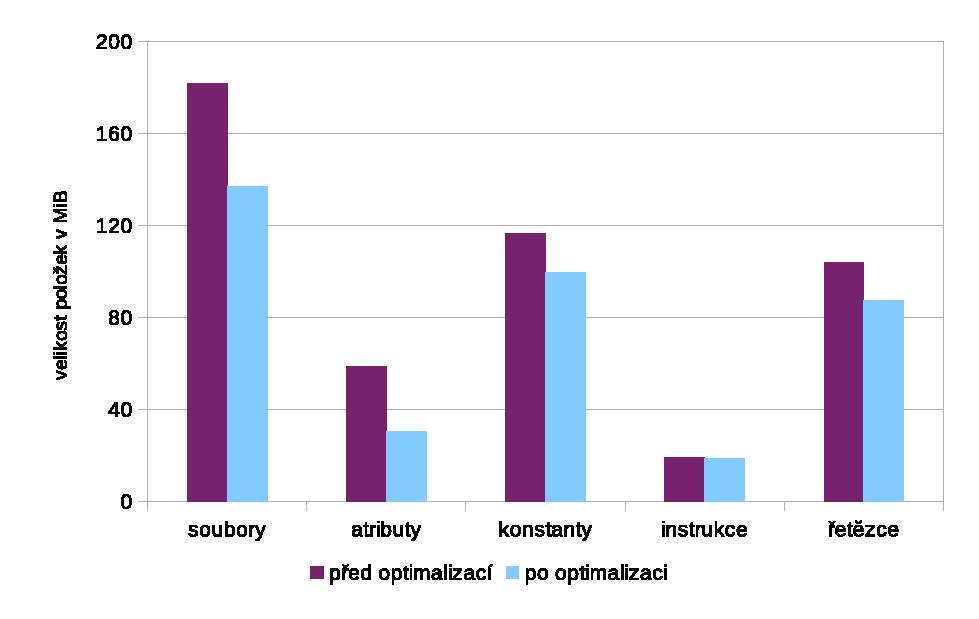
\includegraphics[scale=0.9]{fig/size_comparison}
\caption{Velikosti položek \texttt{class} souborů před a po optimalizaci.}\label{fig:cmp_size}
\end{figure}


